% !TEX root = ../presentation.tex
% LLVM

% \begin{slide}{}
%   \only<1>{\vspace{-0.18cm}}
%   \only<7->{\vspace{0.6cm}}
%   {
%     \color{llvmblue}\fontsize{70}{70}\selectfont
%     \hspace{0.5cm}LLVM
%   }
%   \vspace{0.9cm}
%
%   {
%     \fontsize{16}{16}\selectfont
%     \color{Red}
%     \only<2-5>{
%       \onslide<2->{Low}\hspace{0.2cm} %
%       \onslide<3->{Level}\hspace{0.2cm} %
%       \onslide<4->{Virtual}\hspace{0.2cm} %
%       \onslide<5>{Machine}
%     }
%     \only<6->{
%       \sout{
%         \onslide<2->{Low}\hspace{0.2cm} %
%         \onslide<3->{Level}\hspace{0.2cm} %
%         \onslide<4->{Virtual}\hspace{0.2cm} %
%         \onslide<5->{Machine}
%       }
%     }
%   }
%
%   \vspace{1cm}
%
%   \only<7>{
%     \huge
%     \color{llvmblue}
%     lldb\hs{0.3cm}
%     opt\hs{0.5cm}
%     lld\hs{0.5cm}
%     lljvm\hs{0.3cm}
%   }
%
%   \only<8->{
%     
\includegraphics[scale=0.045]{dragon}\hspace{0.7cm}%
%     
\includegraphics[scale=0.02]{swift}\hspace{0.9cm}%
%     
\includegraphics[scale=0.02]{rust}\hspace{0.9cm}%
%     
\includegraphics[scale=0.068]{tf}
%   }
%
% \end{slide}
%
% \begin{slide}{Compilers}
%   \begin{tikzpicture}[thick]
%     \tikzset{box/.style={
%       draw,
%       rectangle,
%       rounded corners=1pt,
%       inner sep=1cm}
%     }
%
%     % Frontend
%     \onslide<2-4>{
%       \path (0, 0) coordinate [box] (front) node {Frontend};
%     }
%
%     % Optimizer
%     \onslide<3->{
%       \path (4, 0) coordinate [box] (opt) node {Optimizer};
%       \draw [->] (front) -- (opt);
%     }
%
%     % Backend
%     \onslide<4-5>{
%       \path (8, 0) coordinate [box] (back) node {Backend};
%       \draw [->] (opt) -- (back);
%     }
%
%     % Many Frontends
%     \onslide<5->{
%       \path (0,  2.5) coordinate [box] (cpp) node {C\texttt{++}};
%       \path (0,  0) coordinate [box] (go) node {Go};
%       \path (0, -2.5) coordinate [box] (rust) node {Rust};
%
%       % Edges
%       \draw [->, bend left] (cpp) to (opt);
%       \draw [->] (go) -- (opt);
%       \draw [->, bend right] (rust) to (opt);
%     }
%
%     % Many Backends
%     \onslide<6->{
%       \path (8, +2.5) coordinate [box] (x86) node {x86};
%       \path (8,  0) coordinate [box] (arm) node {ARM};
%       \path (8, -2.5) coordinate [box] (riscv) node {RISC-V};
%
%       % Edges
%       \draw [->, bend left] (opt) to (x86);
%       \draw [->] (opt) -- (arm);
%       \draw [->, bend right] (opt) to (riscv);
%
%     }
%   \end{tikzpicture}
% \end{slide}
%
% \begin{frame}[fragile]{LLVM}
%   \begin{center}
%   \begin{tikzpicture}[thick]
%     \tikzset{box/.style={
%       draw,
%       rectangle,
%       rounded corners=1pt,
%       inner sep=0.9cm}
%     }
%     \tikzset{pass/.style={
%       draw,
%       rectangle,
%       rounded corners=1pt,
%       text height=1.3cm,
%       text width=0.25cm}
%     }
%     \tikzset{bigbox/.style={box, inner sep=1cm}}
%
%     %%%%%%%%%%
%     % Frontend
%     %%%%%%%%%%
%     \onslide<1>{
%       \path (0, 0) coordinate [bigbox] (front) node {Frontend};
%     }
%
%     \onslide<2->{
%       \path (0, +1.1) coordinate [box] (lex) node {Lexer};
%       \path (0, -1.1) coordinate [box] (parser) node {Parser};
%       \draw (parser)+(0, -2) node {\texttt{.c,.h}};
%
%       \onslide<-5>{
%         \draw (parser)+(0, -1.5) node {\textbf{Frontend}};
%       }
%       \onslide<6->{
%         \draw (parser)+(0, -1.5) node {\color{Red}\textbf{Frontend}};
%       }
%       \draw [->] (lex) -- (parser);
%     }
%
%     %%%%%%%%%%%
%     % Optimizer
%     %%%%%%%%%%%
%     \onslide<-2>{
%       \path (4, 0) coordinate [bigbox] (opt) node {Optimizer};
%     }
%     \onslide<1>{\draw [->] (front) -- (opt);}
%     \onslide<2>{\draw [->] (parser) -- (opt);}
%
%     \onslide<3->{
%       % Pass blocks and labels
%       \foreach \i/\label/\y %
%         in {0/constprop/-1, 1/licm/+1, 2/inline/-1, 3/loop-unroll/+1} {
%         \draw ({2.75+\i*0.75}, 0) coordinate [pass] (opt\i);
%         \onslide<4->{
%           \draw [dotted, ->]
%                 (opt\i) -- ({2.75+\i*0.75}, {\y * 1.2})
%                 node [pos=1.75] {\label};
%         }
%       }
%
%       % Edges between passes
%       \draw [->] (parser) -- (opt0);
%       \foreach \i/\j in {0/1, 1/2, 2/3} {
%         \draw (opt\i) --  (opt\j);
%       }
%
%       % Optimizer Label
%       \draw (opt)+(0, -2.61) coordinate (opt-label) node {\textbf{Optimizer}};
%       \draw (opt-label)+(0, -0.5) node {\texttt{.ll,.bc}};
%     }
%
%     %%%%%%%%%
%     % Backend
%     %%%%%%%%%
%     \onslide<-4>{\path (8, 0) coordinate [bigbox] (back) node {Backend};}
%     \onslide<-2>{\draw [->] (opt) -- (back);}
%     \onslide<-4>{\draw [->] (opt3) -- (back);}
%
%
%     \onslide<5->{
%       \path (8, +1.1) coordinate [box] (codegen) node {CodeGen};
%       \path (8, -1.1) coordinate [box] (md-opt)
%             node [align=center] {MD\\Optimizer};
%       \draw (md-opt)+(0, -1.5) node {\textbf{Backend}};
%       \draw (md-opt)+(0, -2) node {\texttt{.o,.S}};
%
%       % Edges
%       \draw [->] (opt3) -- (md-opt);
%       \draw [->] (md-opt) -- (codegen);
%     }
%   \end{tikzpicture}
%   \end{center}
% \end{frame}

\begin{frame}[fragile]{clang}
  \begin{lstlisting}[basicstyle=\Large\ttfamily]
            template<typename C>
            struct L {
              char a();
              void n(int) const;
              bool g;
            };
  \end{lstlisting}
\end{frame}

\begin{frame}[fragile]{Clang: Lexer}
    \vspace{0.5cm}
    \begin{lstlisting}[%
      basicstyle=\normalsize\ttfamily,%
      emphstyle=\color{ProcessBlue},%
      emph={C}%
    ]
    template    <   typename    C     >    struct ...
    \end{lstlisting}
    \vspace{-0.65cm}
    \begin{center}
      \scalebox{1.2}{
      \onslide<2>{
      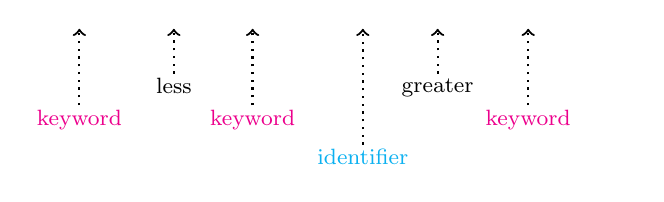
\begin{tikzpicture}[thick, shorten <= -2pt]
        \tikzset{every node/.append style={font=\footnotesize}}

        % template
        \draw [->, dotted] (-6.3, 0)
              node [below] {\color{magenta}keyword}
              -- ++(0, 0.9);

        % <
        \draw [->, dotted] (-5.1, 0.4)
              node [below] {less} -- ++(0, 0.5);

        % typename
        \draw [->, dotted] (-4.1, 0)
              node [below] {\color{magenta}keyword}
              -- ++(0, 0.9);

        % C
        \draw [->, dotted] (-2.7, -0.5)
              node [below] {\color{ProcessBlue}identifier}
              -- ++(0, 1.4);

        % >
        \draw [->, dotted] (-1.75, 0.4)
              node [below] {greater} -- ++(0, 0.5);

        % struct
        \draw [->, dotted] (-0.6, 0)
              node [below] {\color{magenta}keyword}
              -- ++(0, 0.9);

        \node (spacing) at (0.65, 0) {};
      \end{tikzpicture}
      }
      }
    \end{center}
\end{frame}

\begin{frame}[fragile]{Clang: Parser}
\end{frame}

\begin{frame}[fragile]{Clang: Parser}
  \begin{lstlisting}
            void   n   (   int    arg   =   42  )   const  ;
  \end{lstlisting}

  \vspace{-0.3cm}

  \begin{center}
    \onslide<2->{
    \begin{tikzpicture}[thick]
      \tikzset{every node/.append style={font=\ttfamily\footnotesize}}

      % FunctionDecl
      \only<2->{\node (fn) at (0, 0) {\color<2>{brightred}CXXMethodDecl};}

      % Return type
      \only<3->{
        \node (ret) at (-2.5, -1) {\color<3>{brightred}ReturnType};
        \draw [->] (fn) to (ret);
      }

      % isConst
      \only<3->{
        \node (const) at (2.5, -1) {\color<3>{brightred}isConst};
        \draw [->] (fn) to (const);
      }

      % Parameter
      \only<3->{
        \node (param) at (0, -1) {\color<3>{brightred}ParmVarDecl};
        \draw [->] (fn) to (param);
      }

      % Default Argument
      \only<4->{
        \node (default) at (-2, -2) {\color<4>{brightred}DefaultArg};
        \draw [->] (param) to (default);
      }

      % QualType
      \only<4->{
        \node (qualtype) at (0, -2) {\color<4>{brightred}QualType};
        \draw [->] (param) to (qualtype);
      }

      % Identifier
      \only<4->{
        \node (ident) at (2, -2) {\color<4>{brightred}Identifier};
        \draw [->] (param) to (ident);
      }

      % Type
      \only<5->{
        \node (type) at (0, -3) {\color<5>{brightred}Type};
        \draw [->] (qualtype) to (type);
      }

      % CXXRecordDecl
      \only<6->{
        \node (class) at (0, +1) {\color<6>{brightred}CXXRecordDecl};
        \draw [->] (class) to (fn);
      }

      % TranslationUnitDecl
      \only<7->{
        \node (tu) at (0, +2) {\color<7>{brightred}TranslationUnitDecl};
        \draw [->] (tu) to (class);
      }

      % Goes on ...
      \only<8->{
        \draw (default)+(0, -0.5) node {\vdots};
        \draw (ident)+(0, -0.5) node {\vdots};
        \draw (type)+(0, -0.5) node {\vdots};
      }

    \end{tikzpicture}
    }
  \end{center}
\end{frame}

\begin{frame}[fragile]{Clang: IR Generation}
  \pause
  \scalebox{0.8}{
  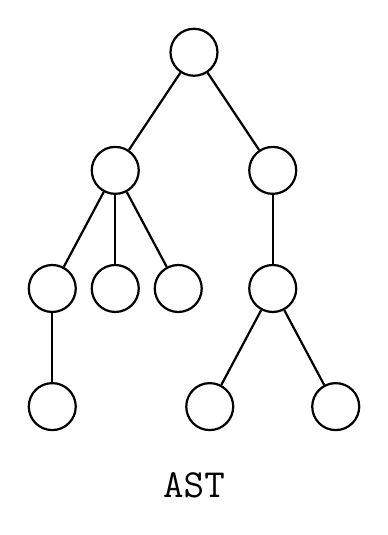
\begin{tikzpicture}[thick]
    \tikzset{node/.style={draw, circle, inner sep=6pt}};

    % AST

    % Root
    \path (0, 0) coordinate [node] (r);

    % Level 1
    \path (-1, -1.5) coordinate [node] (l1a);
    \path (+1, -1.5) coordinate [node] (l1b);

    % Level 2
    \path (-1.8, -3) coordinate [node] (l2a);
    \path (-1.0, -3) coordinate [node] (l2b);
    \path (-0.2, -3) coordinate [node] (l2c);

    \path (+1, -3) coordinate [node] (l2d);

    % Level 3
    \path (-1.8, -4.5) coordinate [node] (l3a);

    \path (+0.2, -4.5) coordinate [node] (l3b);
    \path (+1.8, -4.5) coordinate [node] (l3c);

    % Edges
    \foreach \i in {a, b} { \draw (r) -- (l1\i); }
    \foreach \i/\j in {a/a, a/b, a/c, b/d} { \draw (l1\i) -- (l2\j); };
    \foreach \i/\j in {a/a, d/b, d/c} { \draw (l2\i) -- (l3\j); };

    % Label
    \node at (0, -5.5) {\Large\textbf{AST}};
  \end{tikzpicture}
  }
  \pause
  \hspace{-0.5cm}
  \begin{tikzpicture}[very thick]
    \node at (0, 0) {};

    \node (code) at (4.5, 2.5) [text width=4.6cm, align=justify] {
      \begin{lstlisting}[language=llvm, basicstyle=\fontsize{7.5}{7.5}\ttfamily]
; Function Attrs: nounwind ssp
define i32 @_Z1fi(i32) #0 {
  %2 = alloca i32, align 4
  store i32 %0, i32* %2, align 4
  %3 = load i32, i32* %2, align 4
  ret i32 %3
}
      \end{lstlisting}
    };

    \draw [dotted, ->, shorten >= 10pt, shorten <= -10pt] (0.75, 2.5) -- (code);
  \end{tikzpicture}
\end{frame}
